\section{How precisely is liner exhaustion resolved?}\label{sec:intervals}
We repeated each continuous exposure eight times using the independently
assembled radial nodal system from the sealed sector controller. All 32
runs started cold and advanced to zero phenolic mass. At each refinement we
held the gas load, geometry, chemistry and evolving casing model fixed.
The casing mesh always had one quarter as many radial cells as the liner.

\begin{center}\small\begin{tabular}{lrrrrr}\toprule
& Coarse nodal & Fine nodal & Reference FV & Difference & Gap\\
Motor & [s] & [s] & [s] & [ms] & [ms]\\\midrule
Sustainer Al & 110.576 & 110.482 & 110.474 & +8.6 & 6.4 \\
Sustainer CF & 104.332 & 104.257 & 104.254 & +3.5 & 1.2 \\
Booster Al & 147.746 & 147.623 & 147.610 & +13.6 & 11.3 \\
Booster CF & 138.041 & 137.951 & 137.946 & +4.1 & 1.8 \\
\bottomrule\end{tabular}\end{center}
The coarse column uses the native production settings (80 liner cells,
40~ms maximum step). The fine column uses 640 cells and 2.5~ms. The reference
finite-volume (FV) times use the previously published 640-cell calculation
with a 20~ms maximum step. Each time is the upper end of the final integration
interval. The gap measures the separation between the nearest ends of the two
final intervals. Decimal places here expose differences between calculations.

\begin{figure}[H]\centering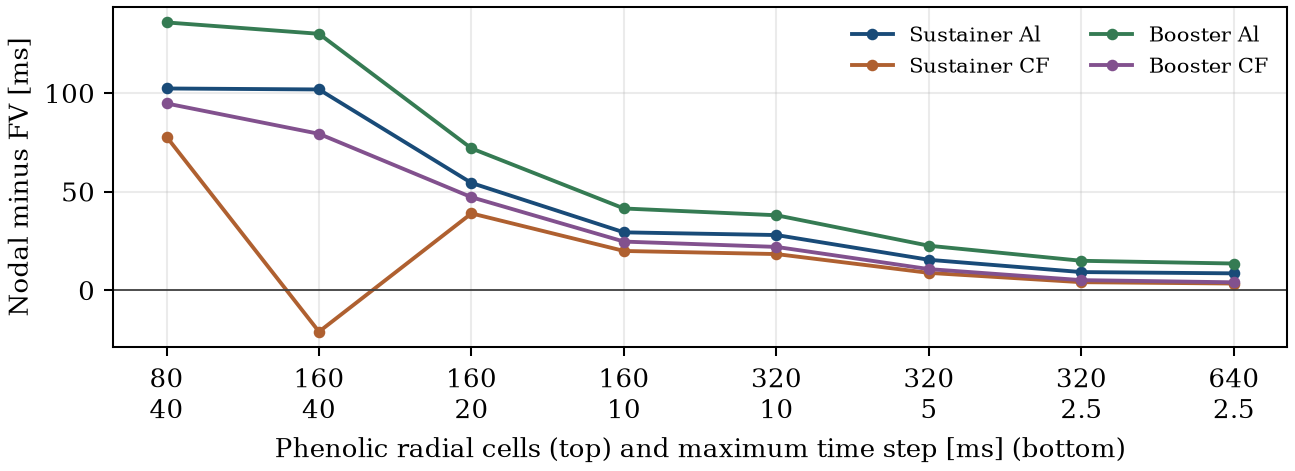
\includegraphics[width=.95\textwidth]{../analysis/whole_event_refinement.png}
\caption{Change in predicted exhaustion time relative to the same FV
reference for each motor. Adjacent settings change either space or time resolution.
The temporary dip for the CF sustainer occurs at the coarse 40~ms step.}
\end{figure}
At 320 liner cells, halving the maximum step from 5 to 2.5~ms changes the
endpoint by at most 7.6~ms. At 2.5~ms, increasing from 320 to 640 cells
changes it by at most 1.4~ms. The fine nodal and reference FV estimates
support the same whole-second scale. The positive gaps still matter for a
claim of tighter agreement. A comparison at matched mesh and time settings
can distinguish residual differences between the two methods from the effect
of their unequal time steps. Material and firing assumptions limit the
physical interpretation throughout.
\clearpage
